\documentclass[a4paper]{article}
\usepackage{ptext}
\usepackage{graphicx}
\usepackage{amsmath}
\usepackage{hyperref}
\usepackage{xepersian}
\settextfont[Scale=.9]{XB Niloofar}
\hypersetup{
 colorlinks=true,
 linkcolor=black,
 urlcolor=blue}






\begin{document}


 \begin{figure}
 \centering
 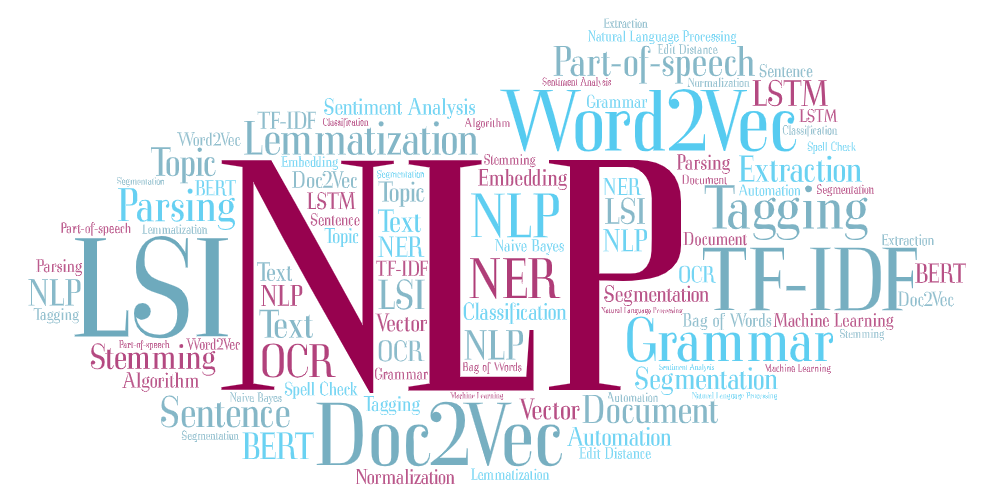
\includegraphics[scale = 0.4]{nlp.png}
 \end{figure}

\title{بسم‌الله الرحمن الرحیم}
\author{گزارش فاز نهایی پروژه درس NLP
\\
نرگس سادات حسینی
\\
لینک دسترسی به پروژه : \lr{\href{https://github.com/nshm99/NLP_Project} {NLP Project}}}
\maketitle
\newpage


\addtocontents{toc}{\textbf{عنوان}~\hfill\textbf{صفحه}\par\rule{\linewidth}{1pt}\par}
\tableofcontents

 
\newpage
\section{بخش \lr{word2vec}}
برای به دست آوردن بردارد کلمات در این قسمت از کتابخانه gensim استفاده شده است. علت استفاده از این کتابخانه و عدم استفاده از تمرین A2 این بود که در تمرین A2 داده ورودی به حالت خاصی بود که تغییر داده‌های موجود به دست‌آمده از فاز قبل به شکل داده‌های تمرین۲ کار وقت ‌گیری بود و به همین علت از کتابخانه آماده برای آموزش مدل استفاده شد.
\newline
برای آموزش مدل، ابتدا مدل اولیه توسط تابع Word2Vec ساخته می‌شود و پارامترهای آن مانند اندازه بردار کلمات مشخص می‌شوند. سپس با استفاده از داده ورودی، کلمات مدل ساخته می‌شوند و درآخر مدل روی داده آموزش می‌بیند. داده‌ای که برای آموزش مدل استفاده شده است، از \lr{combined data word broken.csv} می‌باشد که داده جمع‌آوری شده و پردازش شده از فاز قبل است که به کلمات شکسته شده‌است. مدل‌های آموزش دیده در پوشه models ذخیره می‌شوند.
\newline
پس از آموزش مدل، بردار تعدادی از کلمات پرتکرار مشترک بین دو برچسب رسم شده است که به صورت زیر می‌باشد:
\newline
‎\graphicspath{{../reports}}‎

\begin{figure}[h!]
\centering{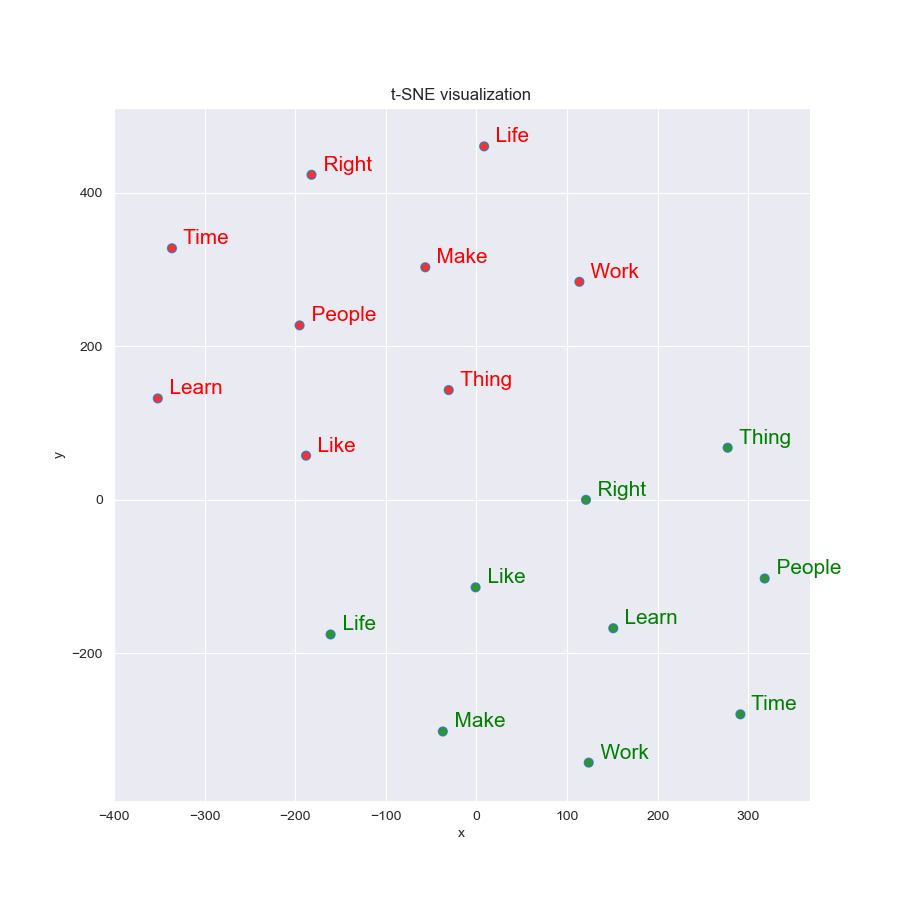
\includegraphics[width=\linewidth]{word_vectors_common.png}}
\caption{بردار کلمات مشترک}
\label{f1}
\end{figure}
\vspace{10mm}
همانطور که مشخص می‌باشد بردار یک کلمه در هر لیبل متفاوت می‌باشد(تقاط سبز برای برچسب motivational و نقاط قرمز برای برچسب nonMotivational می‌باشند). از نظر من علت تفاوت این می‌باشد که هر کلمه در هر برچسب در یک context خاص آمده و به همین علت بردار آن‌ها متفاوت می‌باشد. برای بررسی بیشتر دو کلمه به طور جداگانه بررسی شداند و همچنین برای فهم بهتر کلمات مشابه با آن کلمات نیز استفاده شده‌اند.
\newline
در مثال اول بردار کلمه learn و کلمات مشابه آن برای هربرچسب رسم شده‌است(برای تشابه از تابع \lr{most similar} استفاده شده‌است) . نقاط آبی و سبز برای برچسب motivational و نقاط نارنجی و قرمز برای برچسب nonMotivational می‌باشند.
\newline
\begin{figure}[h!]
\centering{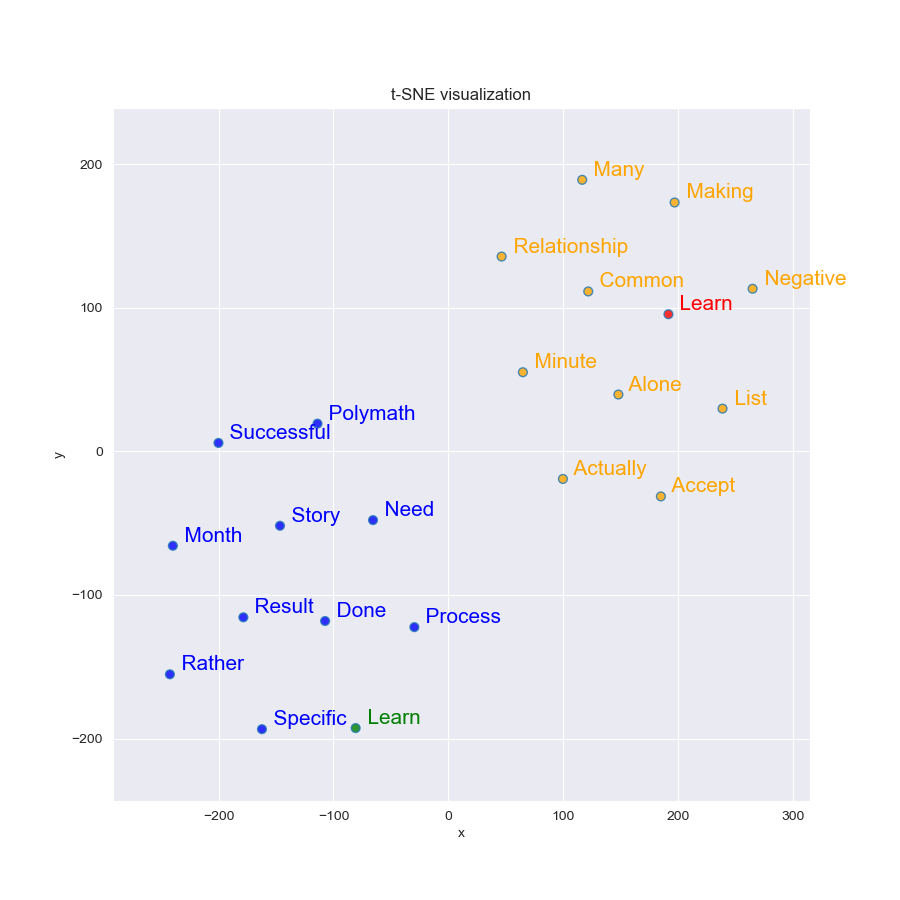
\includegraphics[width=\linewidth]{word_vectors_common_learn}}
\caption{بردار learn}
\label{f1}
\end{figure}
\vspace{10mm}
\newline
با دقت در کلمات نزدیک هر برچسب دیده می‌شود که برای برچسب motivational کلماتی تا حدودی بار مثبت دارند و مفاهیمی همچون process یا انجام دادن را بیشتر می‌رسانند. اما در مقابل کلمات برچسب nonmotivational این بار مثبت را ندارند و تا حدودی می‌توان گفت حتی بار منفی دارند. به طور مثال کلماتی همچون alone می‌توانند تایید‌کننده این موضوع باشند.
\newpage
مثال دوم کلمه right می‌باشد که بردار کلمات به صورت زیر می‌باشد:
\newline
\begin{figure}[h!]
\centering{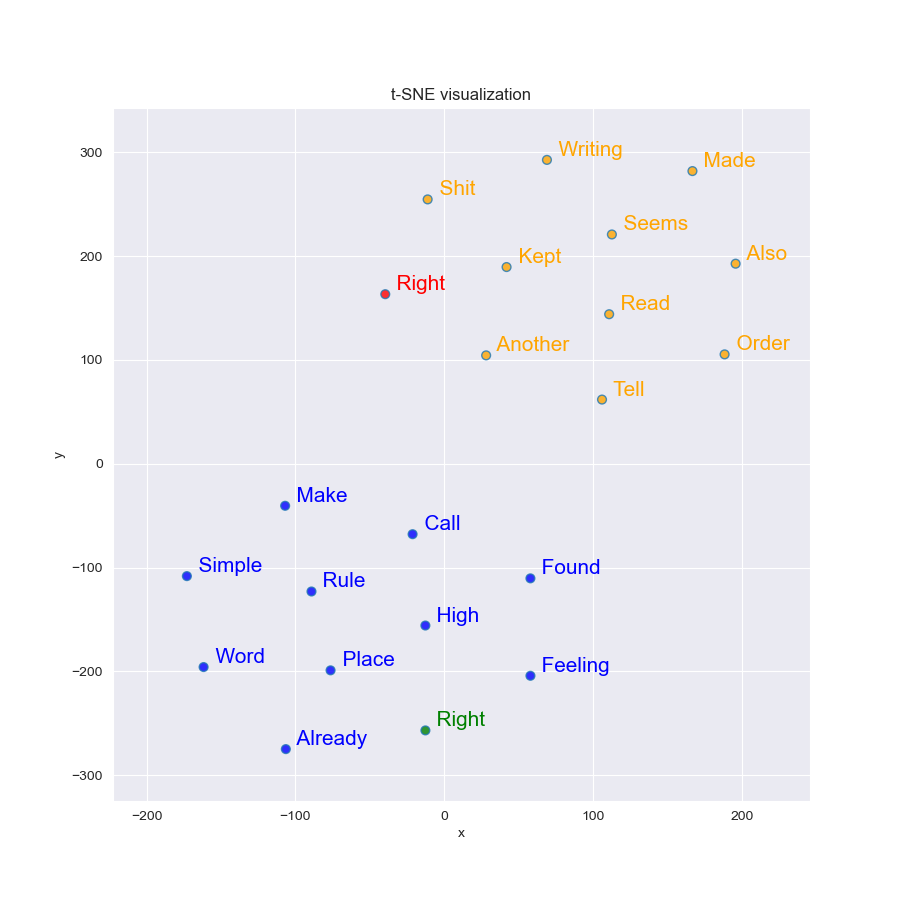
\includegraphics[width=\linewidth]{word_vectors_common_right.png}}
\caption{بردار right}
\label{f1}
\end{figure}
\vspace{10mm}
\newline
در این مثال چیزی که قابل توجه است این‌ می‌باشد که دیگر در این حالت نمی‌توان ادعا داشت که یک کلمه بار مثبت و دیگری منفی دارد(برخلاف مثال قبل). از نظر من علت این‌که کلمه right برای هر دو برچسب تقریبا یک معنی دارد(هرچند بردار آن‌ها با توجه به متفاوت بودن context و این که هر کدام از آن‌ها رو یک مدل آموزش دیده‌اند، متفاوت است) این می‌باشد که بعضی کلمات تنها یک معنی دارند و نمی‌توانند بار مثبت یا منفی بگیرند. به طور مثال کلمه learn که در مثال قبل بود، می‌تواند به معنی آموزش موضوعات جدید برای پیشرفت باشد یا می‌تواند به معنی درس گرفتن از یک اتفاق ناخوشایند پیش‌آمده باشد، اما تمامی معانی کلمه right به گونه‌ای هستند که نمی‌توان این نوع دسته‌بندی برای معانی آن در نظر گرفت.
\newline
برای بررسی بایاس در مدل از تابع \lr{most similar} استفاده شده‌است. یک مثال از بایاس به صورت زیر می‌باشد:
\newline
\newline
\lr{male->sexual = female ->  [('time'), ('feel'), ('assault')]      \newline   female->sexual = male ->  [('assault'), ('survivor'), ('harassment')]
}
\newline
برای پیدا کردن بایاس کلمات متفاوتی انتخاب شدند و با توجه به اینکه همه‌ی داده‌ها از یک موضوع نبودند و جمع چندین موضوع متفاوت بودند، پیدا کردن بایاس کار سختی بود و بعضا خروجی مناسبی تولید نمی‌شد(همانند مثال بالا برای female ) اما در مثال گفته شده بایاس مشخص می‌باشد به این صورت که برای female کلمات مرتبطی را تولید نمی‌کند اما برای male اولین کلمه‌ای که پیدا شده کلمه assault می‌باشد(و دو کلمه دیگر نیز حدودا باهمین مفهوم هستند) که به نظر من این نوعی بایاس می‌باشد که یک بدبینی نسبت به male دربرابر female می‌باشد(مثلا در موضوع assault ) که این بایاس در افکار جامعه و در نتیجه در متن جمع‌‌آوری شده نیز وجود دارد.
\newline
\section{بخش \lr{language model}}
!برای اجرا این بخش با توجه به این‌که به GPU نیاز داشتم کد را در نوت‌بوک زدم و هم فایل نوت‌بوک و هم فایل \lr{.py} آن موجود است.
\newline
برای ساختن \lr{language model} در این بخش از keras استفاده شده است. در مرحله اول داده‌ی هر برچسب به صورت کلمه کلمه به عنوان لیستی از token ها ذخیره می‌شوند. سپس برای هر کلمه یه context به طول length در نظر گرفته می‌شود تا مدل با استفاده از context کلمه بعدی را پیش‌بینی کند. سپس برای انجام محاسبات بعدی  context ذخیره شده(یا sequence) به صورت اعداد int ذخیره می‌شوند.
\newline
سپس ورودی و خروجی مدل برای آموزش بر اساس sequence تولید می‌شود. معماری شبکه به صورت زیر می‌باشد:
\begin{figure}[h!]
\centering{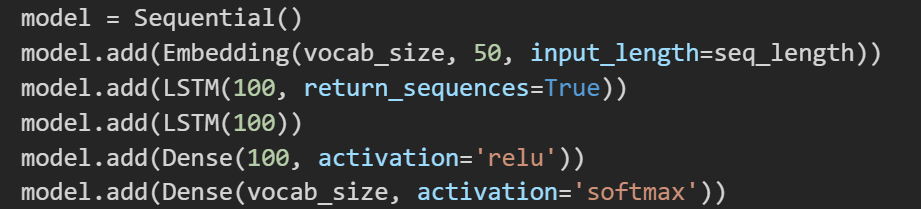
\includegraphics[width=\linewidth]{arch.PNG}}
\caption{معماری شبکه}
\label{f1}
\end{figure}
\vspace{10mm}
\newline
برای بررسی عملکرد شبکه یک متن دلخواه  با طول مشخص به شبکه می‌دهیم . خروجی شبکه برای برچسب nonMotivational  به صورت زیر می‌باشد:
\newline

\lr{[the war between syria and ISIS has affected life of many muslims] pattern toward learn feel suppressing revolution 2000 debt turkey rick describing among able published nation assume military stole appeal ptsd happen quite terrible outline voice blair guardian west administration want attack syria began respected israel imposed mandated dimension since dimension soviet since since since sold continues racism egypt russia rejected}
\newline
وبرای motivational :
\newline
\lr{to be productive you should start state like kinetic applied area hour ratchet impact single midlow receive move mean thing start wish wished quantity single midlow difference mutual time abstract goal time want make life want become going succeed business people want compelled write mean manager total daily people available information large daily year every habit}
\newline

با توجه به متن تولید شده به نظر می‌آید که شبکه کلمات را تقریبا متناسب با برچسب می‌دهد اما جملات تولید شده از نظر قواعد و معنی درست نیستند و به نظر من علت این موضوع این باشد که داده‌ای که مدل روی آن آموزش دیده است مناسب نبوده است، زیرا در مراحل اولیه پردازش داده بسیاری از اطلاعات (به طور مثال puncutaion و stopwrds ) حذف شده‌اند و تنها کلمات به مدل داده شده‌اند. به همین علت جملاتی تولیدی کیفیت مطلوب را ندارند اما می‌توان گفت کلمات تولید شده به درستی و مرتبط با برچسب تولید شده‌اند.
\section{بخش \lr{fine tuning}}
!این قسمت نیز همانند قسمت ۴ در نوت‌بوک نوشته شده است.
در این قسمت برای classification با استفاده از bert ، ابتدا \lr{bert base uncased} که یک \lr{pretrained tokenizer } می‌باشد، load می‌شود.
\newline
سپس داده ورودی به دو دسته آموزش و تست دسته بندی می‌شود(داده ورودی داده پردازش شده و clean شده می‌باشد). سپس tokenizer گفته شده برای tokenize کردن دو داده آموزش و تست استفاده می‌شود.
\\
در مرحله بعد دو داده تست و آموزش به فرمت خاص برای مراحل بعد تبدیل می‌شوند. سپس \lr{pretrained bert classifier} به عنوان مدل آموزش در نظر گرفته می‌شود و آموزش روی آن انجام می‌شود. نتیجه آموزش به صورت زیر می‌باشد:
\begin{figure}[h!]
\centering{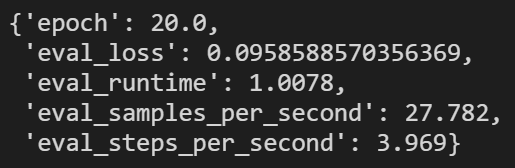
\includegraphics[scale=0.4]{bert_eval.PNG}}
\caption{ارزیابی مدل}
\label{f1}
\end{figure}
\vspace{10mm}
\section{نکاتی درباره کد}
برای قسمت ۴ و ۵ از آنجایی که کد در کولب بود، دیتای موردنیاز دستی آپلود می‌شد(در کد \lr{.py} آدرس‌ها درست است اما در نوت‌بوک باید آپلود شود).
به علت حجم بالای مدل‌ها امکان اپلود آن ها نبود به همین علت لینک درایو آن‌ها را قرار دادم.
\newline
لینک مدل‌های سوال ۴ : \lr{\href{https://drive.google.com/drive/folders/1QlL-aC4LFAVVRrEwDASixCeCh7siHU04?usp=sharing}{language model}}
\newline
لینک مدل سوال ۵ :  \lr{\href{https://drive.google.com/drive/folders/1-8g--A1XqQVx85308QcV9UW5e_yKRojK?usp=sharing}{bert classifier model}}
\newline
مدل‌های قسمت اول نیز در پوشه models قرار دارند.
\newpage

\begin{thebibliography}{9}
\begin{LTRbibitems}

\resetlatinfont
\bibitem{bib1}
\url{https://www.kaggle.com/pierremegret/gensim-word2vec-tutorial}


\bibitem{bib2}
\url{https://stackoverflow.com/questions/43776572/visualise-word2vec-generated-from-gensim}

\bibitem{bib3}
\url{https://towardsdatascience.com/a-beginners-guide-to-word-embedding-with-gensim-word2vec-model-5970fa56cc92}

\bibitem{bib3}
\url{https://medium.com/analytics-vidhya/a-comprehensive-guide-to-build-your-own-language-model-in-python-5141b3917d6d}


\bibitem{bib4}
\url{https://machinelearningmastery.com/how-to-develop-a-word-level-neural-language-model-in-keras/}

\bibitem{bib5}
\url{https://huggingface.co/transformers/training.html}
\end{LTRbibitems}
\end{thebibliography}
\end{document} 